% Problem Statement and Learning Objectives for Chapter 08
\paragraph{Problem Statement}

Motion planning is the process of finding a collision free path between two configurations of a manipulator, considering the presence of obstacles in the workspace.  

\begin{figure}\centering
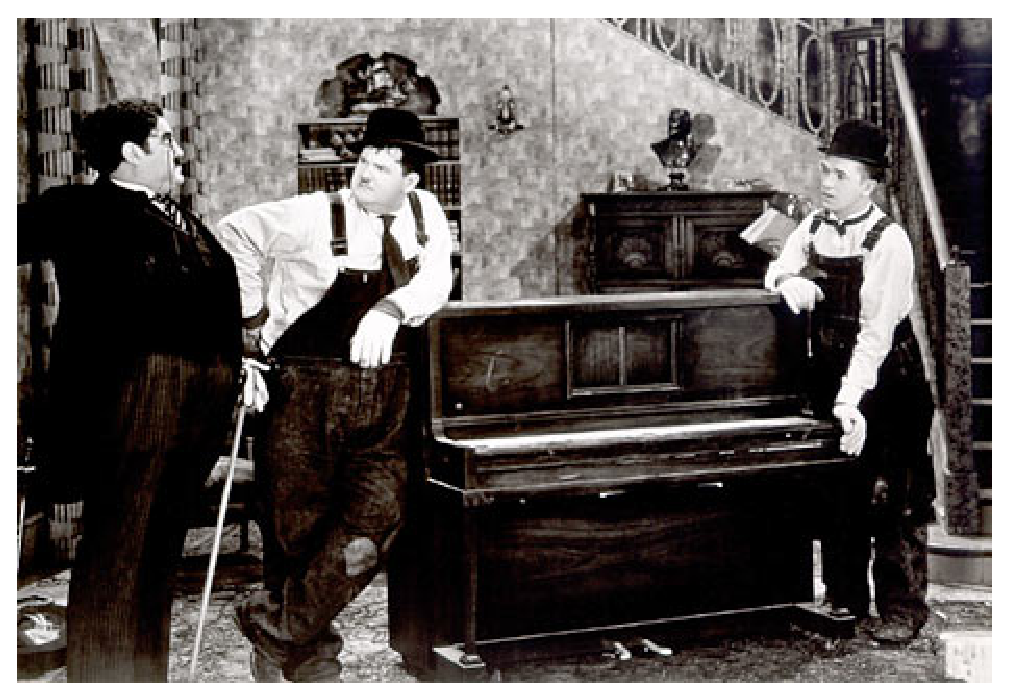
\includegraphics[width=3.5in]{figs08/LaurelHardyPiano.eps}
\caption{How to move the piano up the stairs without touching the walls?}\label{laurelhardy}
\end{figure}

Interestingly, this type of motion planning is usually very easy and natural for humans.  One exception is the case of moving a large bulky object such as a piano through small hallways and doors into a desired room.   This ``piano mover's problem" is similar to the motion planning problem we have posed above.  However if the object (piano) were being manipulated by a (large) serial robot arm, we would also have to consider all potential collisions between the arm and the environment, in addition to the collisions between the piano and the environment. 

\paragraph{Learning Objectives}
Upon completing this Chapter, the reader should be able to
\begin{itemize}
  \item Explain the major problems in motion planning
  \item Identify which ones are most computationally time consuming in typical manipulation applications. 
  \item Explain the Configuration Space.
  \item Describe some sampling based motion planning methods. 
\end{itemize}